% -----------------------------------------------------------------------------
%   Arquivo: ./02-elementos-textuais/metodologia.tex
% -----------------------------------------------------------------------------

\chapter{Desenvolvimento do trabalho}
\label{chap:metodologia}

\begin{comment}
 proposta: reconstruir um software desde a sua arquitetura
 justificativa: paradigama de atores incompatível com o modelo de threads
 metodologia: 
  -- analisar os pontos criticos da atual versão para fins de estabelecer a forma mais adequada de fazer a migração
  -- particionar o software 
  -- como  o software consiste em cadeias de estimulação, optou por fazer cada circuito completo sensório-motor 
  -- para cada circuito implementado, o funcionamento sera verificado e validado
  -- criterio usado para escolha dos circuitos 
  -- para cada circuito será gerada uma versão da arquitetura
  -- na ultima versão, realizar experimentos computacionais a fim de verificar se os resultados produzidos pela nova arquitetura são compatíveis com os já obtidos anteriormente
\end{comment}

Como abordado no \autoref{chap:fundamentacaoTeorica}, o modelo de programação concorrente clássico é incompatível com o modelo de atores. Enquanto no primeiro a comunicação é feita utilizando compartilhamento de memória, o que pressupõe sincronização no acesso compartilhado, o segundo abre mão dessa possibilidade, estabelecendo a troca de mensagens assíncrona como forma de comunicação, assumindo que as unidades de processamento podem não estar na mesma máquina.

Neste sentido, o presente capitulo apresenta a modelagem de um simulador, baseado no modelo de atores, escolhendo o modelo de sistema nervoso artificial apresentado pela arquitetura Artífice. A próxima seção descreve a metodologia adotada, a modelagem dos sistemas internos da criatura está descrita na \autoref{sec:criatura}. Estabeleceu-se um protocolo para comunicação entre componentes em diferentes nós, descrito na \autoref{sec:cluster}. 

\section{Metodologia}
\label{sec:metodologia}

A proposta principal do presente trabalho é construir simulador de criaturas artificiais interagentes, cada qual dotada de sistema nervoso, baseado no modelo de atores e que opere como um AD-MAS - \textit{Asynchronous Distributed Multi-Agent System}. Usar esta tecnologia se justifica pelo fato de que assincronia intrínseca do modelo de atores favorece a escalabilidade e se adéqua bem ao modelo de sistema nervoso escolhido. Dado este objetivo, para desenvolver um software distribuído é necessário> particioná-lo em componentes que devem executar no mesmo espaço de endereçamento e naqueles que podem executar em espaços distintos; projetar os algoritmos de sincronização e propagação de informação no \textit{cluster}.  

No modelo de sistema nervoso artificial escolhido, a arquitetura Artífice, existem duas entidades principais: as criaturas artificiais e os componentes do mundo, com os quais a criatura interage. Uma criatura é composta de vários componentes internos que interagem entre si através de troca de estímulos, formando cadeias de estimulação. Portanto o primeiro passo para produzir uma nova implementação utilizando o modelo de atores foi identificar os componentes e estímulos trocados, e implementar cada uma das cadeias de estimulação. Para cada circuito implementado, uma versão da arquitetura deve ser gerada, e seu funcionamento  testado e validado. 

Um mecanismo de extração e análise de dados deve ser implementado. Ao finalizar a implementação de todas as cadeias de estimulação, experimentos computacionais devem ser realizados, coletando-se dados do funcionamento para comparar com os resultados anteriores. Portanto a criatura deve ser capaz de salvar dados da dinâmica interna em banco de dados, de forma que seja possível recuperá-los para analise posterior. 
Em resumo, a metodologia proposta segue: 

\begin{enumerate}
\item identificar os componentes da criatura e as trocas de estímulos e as cadeias de estimulação

\item implementar cada uma das cadeias, testando o funcionamento de cada uma delas

\item desenvolver um esquema de banco de dados relacional para salvar os dados da simulação

\item propor e implementar um modelo de distribuição dos componentes, bem como os algoritmos de sincronização

\item propor e executar um conjunto de experimentos computacionais para validar o software produzido, verificando o seu correto funcionamento e a sua escalabilidade
\end{enumerate}

A \autoref{sec:criatura} contempla o desenvolvimento dos itens 1, 2 e 3 da metodologia, enquanto a \autoref{sec:cluster} contempla o desenvolvimento do item 4. A descrição detalhada dos experimentos enumerados no item 5 e os resultados obtidos encontram-se no \autoref{chap:resultados}.

\section{Dos componentes da criatura e da dinâmica interna}
\label{sec:criatura}

Nesta sessão se propõe a discussão da modelagem da dinâmica interna de uma criatura artificial baseando-se na proposta pela arquitetura Artífice. Para que não haja confusão entre o primeiro e o segundo modelo, adotar-se-á o nome DL2L \footnote{L2L é acrônimo para a frase \textit{Learn to live, live to learn}, e a letra "D" de distribuído.} para a arquitetura proposta neste trabalho.

Uma criatura artificial é um conjunto de vários componentes que juntos desempenham a dinâmica interna e podem ser divididos em três grandes categorias: os que fazem parte do sistema somático (SS) e compõe estruturas físicas da criatura (corpo, olho, boca, etc.) e portanto tem uma representação geométrica no mundo artificial e trocam estímulos diretamente com este; os que fazem parte do Córtex Sensório-Motor (CSM), que fazem a interface entre o sistema somático e o sistema nervoso central e, por fim, o Sistema Nervoso Central (SNC) que compreende o processo cognitivo-emocional. Os componentes funcionam concorrentemente e trocam mensagens assíncronas. 

Existem outros sistemas que compõe a criatura, como o sistema de memória (SM), o sistema de condicionamento (SC), e o sistema emocional (SE) e o seletor de ação (AS), mas estes não atuam diretamente para a dinâmica interna, mas são utilizados pelo SNC para manter a homeostase, decidir e avaliar as ações da criatura. 

\begin{figure}
    \centering
    \caption{Ciclos de estimulação internos da criatura artificial. O tipo do estímulo emitido pelo componente está descrito no lado esquerdo da seta. Os componentes estão discriminados pela sua classe, segundo a legenda.}
    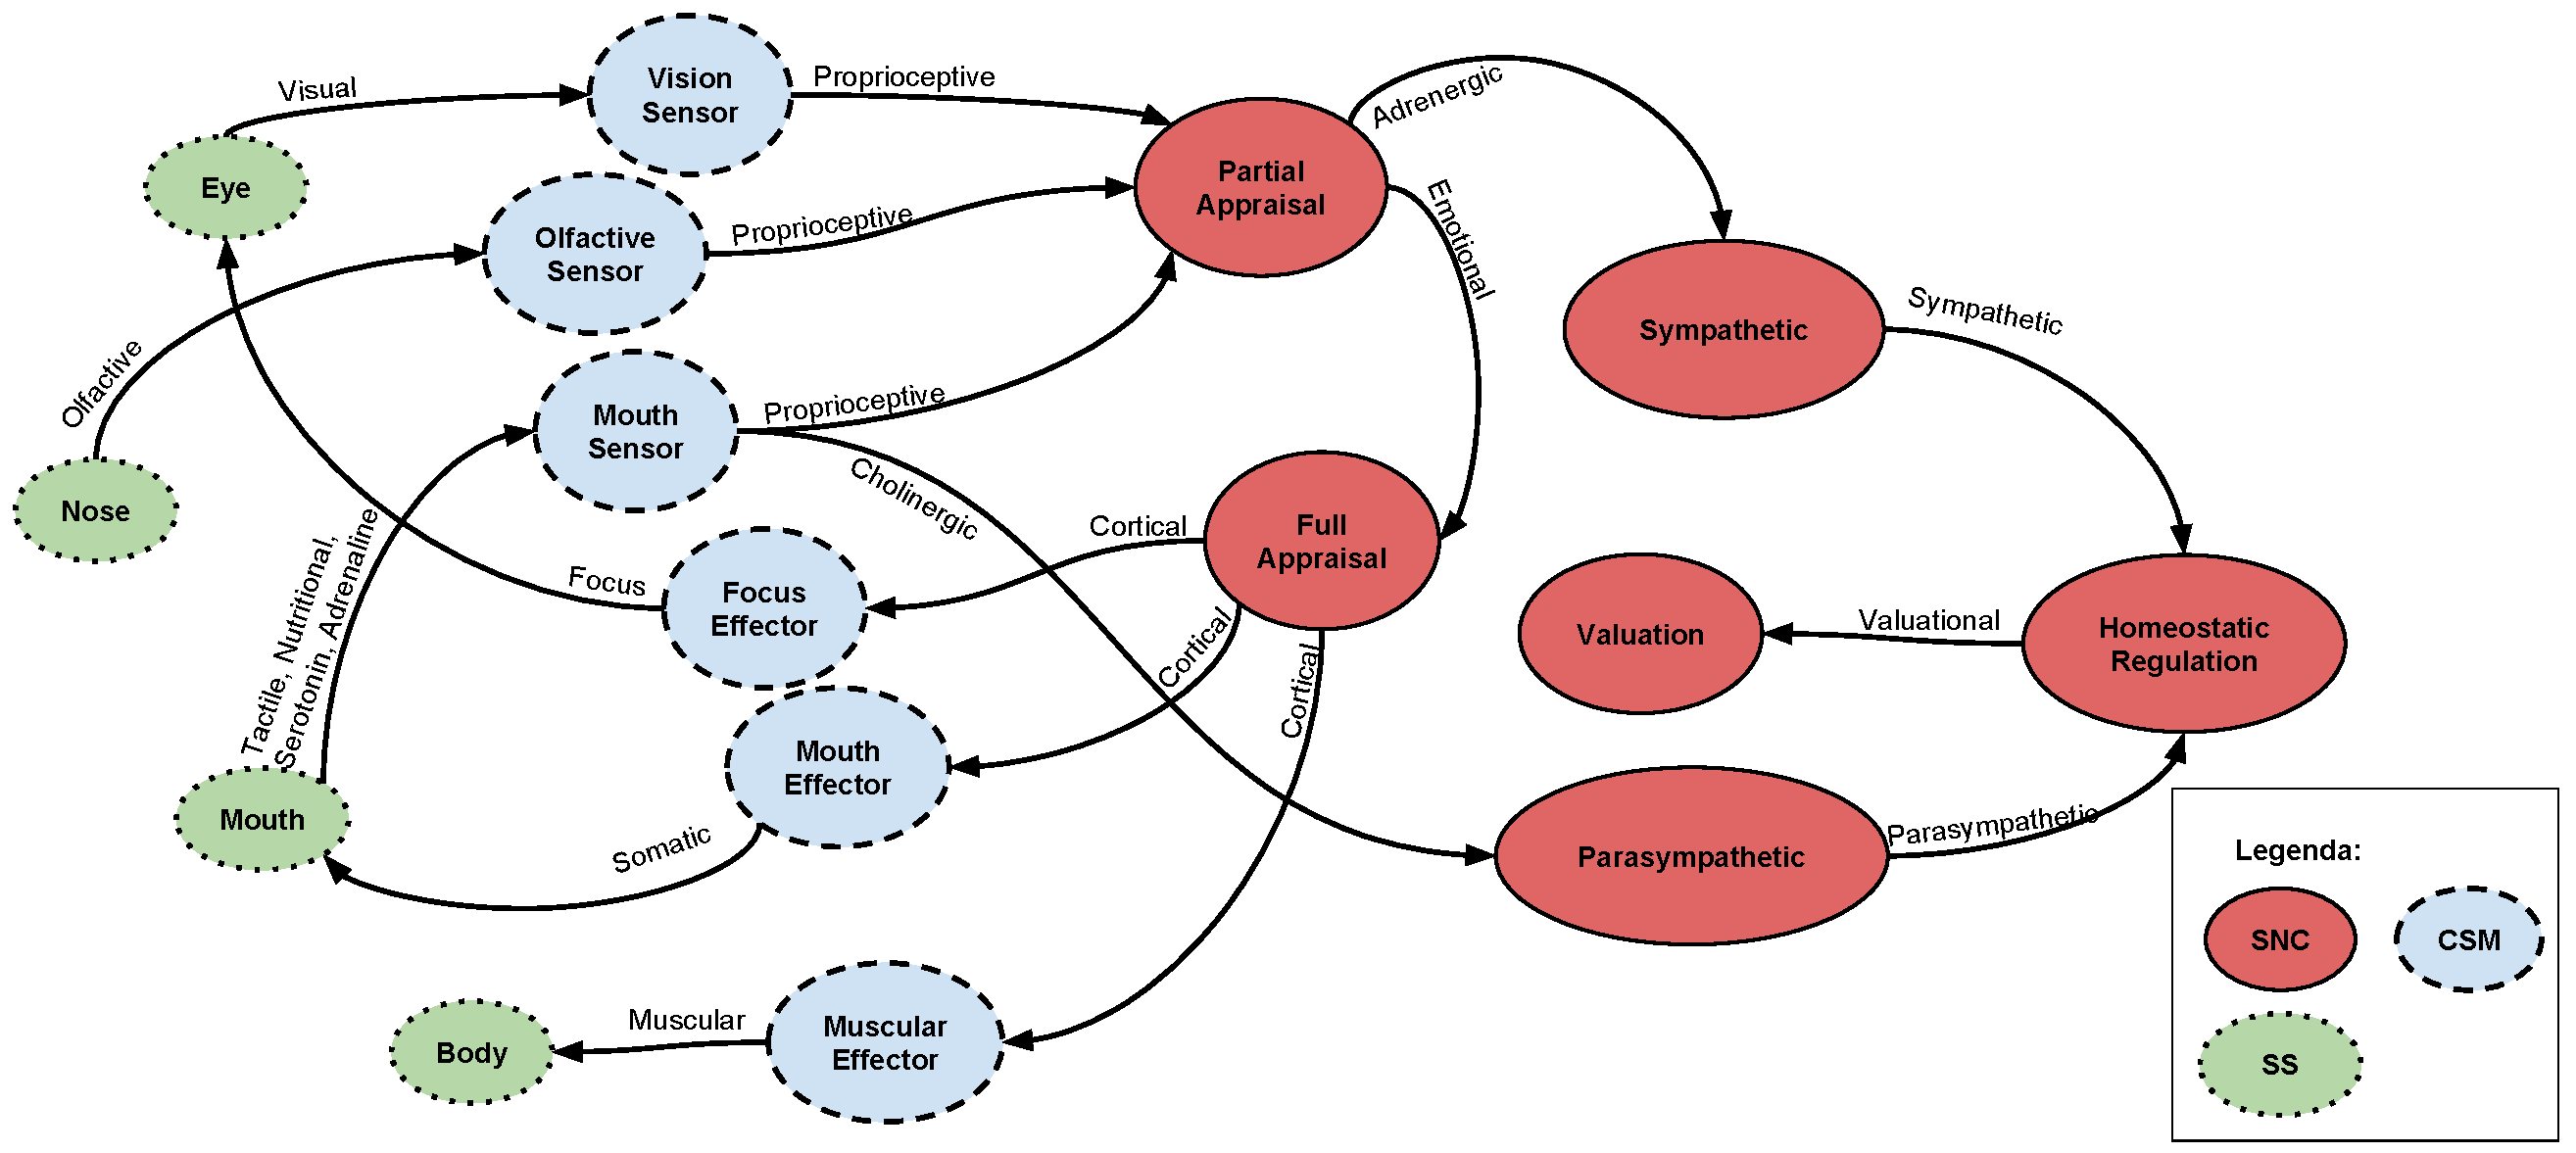
\includegraphics[angle=90,scale=0.5]{./04-figuras/Fig1_CadeiaEstimulos}
    \fonte{O próprio autor}
    \label{fig:cadeiaEstimulos}
\end{figure}

Alguns componentes precisam esperar um certo conjunto de estímulos para funcionar, \textit{e.g.} os que integram o córtex sensório-motor, só podem enviar estímulos ao sistema nervoso central uma vez que o sistema somático tenha informado haver algum objeto no campo sensório da criatura. Componentes do SNC por sua vez não precisam aguardar estímulos o tempo todo, que é o caso do \textbf{PartialAppraisal} que faz a avaliação emocional.  A \autoref{fig:cadeiaEstimulos} exibe a cadeia de estímulos trocados entre os componentes internos da criatura artificial. 

A criatura interage com o mundo artificial, através dos seus componentes do sistema somático, a fim de manter a sua regulação homeostática, \textit{i.e.}, manter o nível de excitação de suas emoções em um  valor estável. Para ilustrar o funcionamento da dinâmica interna, será oferecida uma descrição hipotética da sequência de eventos que acontecem quando um objeto entra em seu campo de visão. A descrição abaixo apresentada foi inspirada na proposta por \citeonline{Campos2015} e serve apenas para fim explicativo uma vez que a troca de estímulos é assíncrona e não determinística. Com isso em mente, supondo que a criatura está caminhando pelo mundo quando dois nutrientes A e B entram em seu campo de visão, e olfativo, ambos em contato com a sua boca: 

\begin{enumerate}
    \item o componente \textbf{Eye} receberá dois estímulos do tipo \textbf{Luminous}, um para cada nutriente. E enviará, para cada um deles, um estímulo do tipo \textbf{Visual} para o\textbf{ VisionSensor};
    \item O componente \textbf{Nose} receberá, concorrentemente um estímulo do tipo \textbf{Smell} para cada nutriente, e enviará para o \textbf{OlfactiveSensor} dois estímulos do tipo \textbf{Olfactive};
    \item o componente \textbf{Mouth} receberá dois estímulos do tipo \textbf{Mechanical} e enviará dois estímulos do tipo \textbf{Tactile} ao \textbf{MouthSensor}; 
    \item Os componentes sensores (\textbf{MouthSensor}, \textbf{VisionSensor} e \textbf{OlfactiveSensor}) ao receberem os estímulos citados, produzirão para cada um deles um estímulo do tipo \textbf{Proprioceptive}, que será enviado ao \textbf{PartialAppraisal}, esses estímulos podem chegar juntos ao componente \textbf{PartialAppraisal} ou não;
    \item Supondo que o \textbf{PartialAppraisal} recebe todos os seis estímulos proprioceptivos, ele criará uma situação, que representa o conjunto de sensores ativados e por quais componentes. Essa situação será enviada juntamente com a emoção mais desregulada ao componente \textbf{FullAppraisal}. Supondo que essa emoção seja a fome, ela será utilizada para calcular a eficiência comportamental da criatura. O \textbf{PartialAppraisal} também envia um estímulo do tipo \textbf{Adrenergic} ao componente \textbf{Sympathetic}, dizendo que o \textit{arousal} das emoções deve ser atualizado;
    \item O componente \textbf{Sympathetic} envia um estímulo ao \textbf{HomeostaticRegulation} para atualizar o \textit{arousal} de todas emoções, somando uma constante que será chamada de delta simpático $ \Delta_{sym} $;
    \item o \textbf{FullAppraisal}, ao receber o estímulo do tipo \textbf{Emotional}, criará uma lista de possibilidades de ações, ou \textit{affordances}, que no caso são: comer o nutriente A, comer o nutriente B, evitar os nutrientes, andar em qualquer direção ou dormir. Essa lista, juntamente com a emoção mais desregulada, será enviada ao AS para escolher a próxima ação a ser executada que melhor regula a emoção fome. O AS utiliza os sistemas condicionamento e memória para desambiguar o conjunto de ações, caso não seja possível ele escolhe uma ação aleatória do conjunto de \textit{affordances}.  Assumindo que a ação de comer o nutriente A será escolhida, o \textbf{FullAppraisal} envia para os componentes do córtex efetor  (\textbf{FocusEffector}, \textbf{MouthEffector} e \textbf{MuscularEffector}) em um estímulo cortical essa informação;
    \item O estímulo cortical recebido no \textbf{MouthEffector} é transmitido ao componente \textbf{Mouth} por uma mensagem do tipo \textbf{Somatic} e ao ser recebida no orgão efetor, desencadeia um estímulo destrutivo ao nutriente A;
    \item Os outros componentes do córtex efetor atualizam, nos seus respectivos membros do sistema somático, o valor da eficiência comportamental, que é utilizada para calcular os parâmetros de sensibilidade (dimensão do campo visual, olfativo, tamanho do passo, etc.);
    \item Ao receber uma mensagem destrutiva, o nutriente se remove do mundo e envia à criatura que o destruiu um estímulo nutritivo;
    \item O componente \textbf{Mouth}, recebendo o estímulo nutritivo envia um estímulo do tipo \textbf{Nutritional} para o \textbf{MouthSensor};
    \item O sensor, ao receber o estimulo nutricional, envia ao \textbf{Parasympathetic} um estímulo \textbf{Cholinergic};
    \item O estímulo \textbf{Cholinergic} é recebido no \textbf{Parasympathetic} que encaminha ao \textbf{HomeostaticRegulation} informando que o \textit{arousal} da emoção fome deve ser diminuído. Essa diminuição é igual ao valor nutritivo do estímulo recebido;
    \item O \textbf{HomeostaticRegulation} envia uma mensagem ao \textbf{Valuation} informando que o nutriente já foi comido e a emoção já regulada, e a ação que produziu essa regulação deve ser valorada;
    \item O \textbf{Valuation} atualiza a memória de condicionamento e a memória de longo prazo ao receber uma mensagem do \textbf{HomeostaticRegulation} e o ciclo de estimulação termina neste passo.
\end{enumerate}

É importante ressaltar que o processamento dos estímulos acontece de  maneira concorrente,  e essa é só uma das possíveis ordens de execução. Ademais, o início de um novo ciclo em algum outro componente não influencia o que já está em execução, podendo produzir comportamentos distintos.

Dada a organização entre os componentes da criatura, a estratégia escolhida  para implementá-la  foi criar um ator tipado\footnote{Atores em Akka podem ser não tipados (como nos exemplos do capítulo anterior) ou tipados. Atores tipados devem implementar alguma interface e são acessíveis através e somente dela, como objetos convencionais, mas com as mesmas propriedades de atores convencionais. Para maiores detalhes de implementação, a documentação se encontra em \url{http://doc.akka.io/docs/akka/current/scala/typed-actors.html}} cujo sub-atores criados são seus componentes internos. A hierarquia dos objetos é de um único nível, de forma a facilitar a um componente acessar a referência para outro componente. 

Como os atores de Akka tratam uma única mensagem por vez e o modelo de sistema nervoso do Artífice prevê que um componente deve ser capaz de tratar mais de um estímulo ao mesmo tempo, foi necessário estender a \textit{mailbox default} do \textit{toolkit}, mudando o seu comportamento ao desenfileirar. Na nova implementação, ao ser solicitada a próxima mensagem, o método empacota todas as mensagens que estão na fila em uma lista e entrega essa lista ao ator. Esse novo comportamento cria uma dificuldade ao ator destinatário, que não saberá a referência do remetente de cada mensagem a partir do método \textbf{sender()}, uma vez que os estímulos são desempacotados de seus envelopes que contém essa informação, e empacotados em um novo envelope sem remetente. Entretanto, todo estímulo enviado possui dois identificadores do tipo \textbf{SequentialId} que mantêm o \textit{id} do remetente e do destinatário. Para recuperar o ator que enviou a mensagem, o ator da criatura, que supervisiona os componentes, mantêm uma tabela \textit{hash} que mapeia \textbf{SequentialId}s para o \textbf{ActorRef} do componente.

O \textbf{PartialAppraisal} é um tipo especial de componente, que  precisa exibir um comportamento ativo, enviando estímulos ainda que não tenha recebido nenhum. Como os atores de Akka são reativos, no sentido de que só são executados ao receber uma mensagem de outro ator, é necessário utilizar algum artifício que faça o \textbf{PartialAppraisal} executar periodicamente. Para foi criada uma tarefa no \textit{scheduler} de cada criatura que envia uma uma mensagem para o componente periodicamente. Assim, ainda que não haja nenhuma mensagem vinda do córtex sensor o componente será escalonado de tempos em tempos para tratar, ao menos, essa mensagem. 

Por fim, um ponto importante da implementação das criaturas artificiais é a comunicação com o banco de dados. Ela deve acontecer sempre que um componente terminar sua execução, persistindo dados importantes para analise posterior. Esses dados em geral são o estado de cada componente, o conjunto de estímulos que ele recebeu e que alterou seu estado interno, e o conjunto de estímulos que ele emitiu ao alterar esse estado. A tecnologia utilizada para criar as tabelas do banco de dados e fazer o acesso durante a simulação foi a \textit{Java Persistence API} (JPA). Ela foi escolhida para manter compatibilidade com versões anteriores da arquitetura Artífice. 

O diagrama de classes que são persistidas em banco de dados está representado na \autoref{fig:bd}. É possível ver na figura que todos os objetos que representam algum estado relevante durante a simulação estão associados a um \textbf{ChangeStimulusState}. Esta entidade de banco de dados é de grande importância pois é responsável por manter as transduções de estímulos. A saber, uma transdução é a transformação de estímulo que recebido em um estímulo emitido, produzindo uma mudança de estado interno em um componente. Toda alteração de estado é salva com o \textit{timestamp} em que ela aconteceu e, juntamente com a entidade \textbf{StimulusState}, forma um grafo pelo qual é possível reconstruir a cadeia de estimulação que produziu um comportamento qualquer da criatura artificial. 

É relevante  saber o instante em que os componentes alteraram seu estado uma vez que este modelo cognitivo se comporta como um sistema dinâmico no tempo, e a maioria das análises são feitas baseadas nele. Além disto, como este é um sistema inteligente que deve exibir um comportamento coerente, é necessário também correlacionar a dinâmica externa da criatura artificial com seu estado interno. A título de exemplo, é preciso saber se a criatura come quando sua emoção mais desregulada é a fome, ou qual mecanismo de decisão ele usa para desambiguar uma ação.  

\begin{comment}
 -- timestamp em  tudo, como é um sistema assincrono
 -- um sistema com um grau de inteligencia é necessário correlacionar os dados da dinamica interna e externa 
 -- retirar as informações necessarias pra reconstruir grafico da dinamica interna e externa
 -- dar um exemplo, queremos saber se estando com fome ele opta por decidir comer algo ou fazer outra 
\end{comment}

\begin{figure}
    \centering
    \caption{Diagrama de classes do banco de dados}
    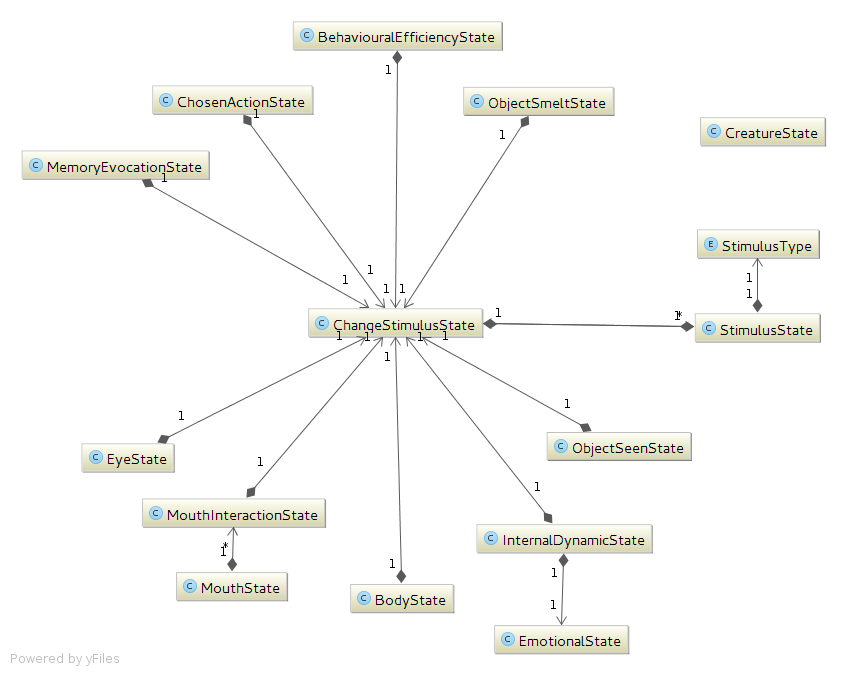
\includegraphics[scale=0.55]{04-figuras/bd.png}
    \fonte{O próprio autor}
    \label{fig:bd}
\end{figure}

\section{Dos componentes da simulação em ambiente distribuído}
\label{sec:cluster}

Ao particionar o funcionamento da arquitetura Artífice, foram identificados quatro papéis importantes que podem funcionar de modo distribuído, eles são: o gerenciamento da simulação; gerenciamento dos componentes da simulação (criaturas e nutrientes); o fornecimento de identificadores, e a manutenção física da simulação. Para cada uma das responsabilidades apresentadas foram projetados um ator e suas peculiaridades serão descritas adiante. A \autoref{fig:cluster} mostra um esquema de como os atores se organizariam com $K$ \textit{holders}, $M$ criaturas e $N$ nutrientes. Este esquema é um dos muitos possíveis que poderiam ser adotados e foi escolhido tendo em vista o balanceamento de criaturas e nutrientes ao longo dos nós de processamento, entretanto, outras possibilidades de organização devem ser estudadas em trabalhos futuros, analisando a performance em termos de sistemas distribuídos, bem como a mudança desse esquema de distribuição influencia o comportamento das criaturas.

\begin{figure}
    \centering
    \caption{Esquema de nós do \texit{cluster}. Os atores conectados por linhas pontilhadas podem executar em máquinas separadas enquanto os atores conectados por linhas contínuas estão subordinados, devendo executar no mesmo computador que seus supervisores. As linhas pontilhadas portanto indicam que a comunicação acontece via rede, enquanto as linhas contínuas indicam que a comunicação acontece sem o uso da rede}
    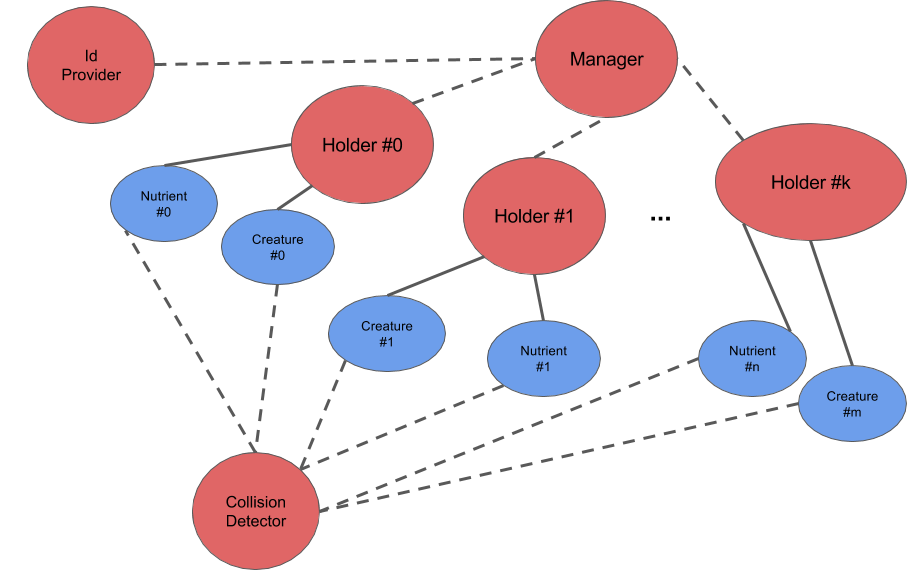
\includegraphics[scale=0.5]{04-figuras/cluster.png}
    \fonte{O próprio autor}
    \label{fig:cluster}
\end{figure}

Para auxiliar na comunicação de atores em diferentes processos foi utilizada a biblioteca \textit{akka-cluster} \footnote{\url{http://doc.akka.io/docs/akka/current/java/common/cluster.html}} que faz parte do \textit{toolkit} Akka. Ela oferece um serviço descentralizado de adesão de atores, distribuídos em vários processos ao longo da rede. A biblioteca permite identificar quando novos membros entram na rede ou saem dela. Ela é baseada no protocolo \textit{gossip} e possui um detector automático de falhas, oferecendo um serviço sem ponto único de falha ou ponto único de gargalo.

O ator responsável pelo gerenciamento da simulação, o \textit{manager}, tem o papel de iniciar e interromper a simulação, fazendo interface com o usuário final. Ele mantém uma tabela com a referência de todos os nós associados a uma simulação, e é responsável por entregar um identificador a todo novo nó  do tipo \textit{holder} que entra no \textit{cluster}. Esse identificador será necessário para encontrar de forma eficiente um membro da simulação em um nó do \textit{cluster} partindo de outro nó qualquer. Ao receber uma notificação que um nó importante falhou, a simulação é imediatamente interrompida pelo \textit{manager}. 

Como os identificadores do tipo \textbf{SequentialId} são globais para toda a simulação, optou-se por gerá-los de forma centralizada, garantindo que não existam dois identificadores repetidos. Essa estratégia foi adotada por ser a que teria menor \textit{overhead} de implementação. Tratar a falha do \textit{id-provider}, ator responsável por gerar os identificadores, é simples de corrigir: reinicia-se o ator em outro nó. O \textit{manager} deve ter conhecimento do \textit{id-provider} mas não é necessário mantê-lo indexado.

As colisões entre os objetos da simulação continua sendo verificada por um nó centralizado chamado \textit{Collision Detector}. Esse nó recebe mensagens constantemente, sempre que uma criatura atualiza sua posição ou um nutriente é destruído, e deve responder, a cada nova mensagem, com quais objetos o remetente colidiu. O algoritmo de pesquisa que encontra o conjunto de objetos com o qual o remetente da mensagem colidiu é sequencial e linear no número de objetos no mundo, o que pode ser um gargalo, à medida que o tamanho do mundo cresce. Esta tarefa é de crucial importância para um AD-MAS como este em que, o mundo artificial possui uma representação geométrica e toda a dinâmica de interação entre as criaturas e objetos depende desta representação. Dessa forma, manter a verificação de colisões centralizada em um nó, além de caracterizar um ponto único de falha (o que é um aspecto negativo do ponto de vista de sistemas distribuídos), pode ser prejudicial para o desempenho e escalabilidade, além de levar dinâmica interna das criaturas à degradação. Neste sentido, é importante reforçar a necessidade de avaliar outros modelos de distribuição, levando em conta uma melhor abordagem para o problema de verificar colisões em um sistema distribuído que depende do tempo.  

Finalmente, o \textit{holder} é responsável por manter as entidades da simulação, criaturas e nutrientes. Ele também mantém uma tabela com os outros \textit{holders} que fazem parte do \textit{cluster}. Esse índice é construído dinamicamente à medida em que as criaturas vão trocando estímulos com os objetos do mundo que podem estar em outros \textit{holders}. Ao entrar no \textit{cluster}, um \textit{holder} deve receber um identificador inteiro sequencial do \textit{manager}. Ao receber a informação do usuário que um novo membro deve ser criado, é papel do \textit{manager} solicitar um novo \textbf{SequentialId} ao \textit{id-provider}. O resto da divisão inteira da super-chave do identificador pelo número de \textit{holders} no \textit{cluster} informa em qual \textit{holder} o novo membro deve ser criado. Assim o \textit{manager} ordena a criação do novo membro no nó apropriado. 

As criaturas dentro de um \textit{holder} podem eventualmente querer se comunicar com membros em outro \textit{holder} a partir dos identificadores trocados nas mensagens, sem saber exatamente onde está fisicamente o ator, \textit{e.g.} uma criatura que está no \textit{holder-1} pode querer enviar um estímulo destrutivo para um nutriente que esteja no \textit{holder-2}. Para tanto, a criatura encaminha a mensagem ao seu \textit{holder}: caso ele conheça o nó do destinatário, a mensagem é encaminhada a ele. Caso o \textit{holder} do destinatário seja desconhecido, a mensagem é enviada ao \textit{manager} que a encaminha ao \textit{holder} apropriado e responde com o endereço dele ao \textit{holder} remetente, para  que ele seja indexado. Esse algoritmo é baseado no \textit{plugin} \textit{akka-cluster-sharding}, que oferece a funcionalidade de endereçar um ator por um identificador lógico sem conhecer sua localização física. Optou-se por adotar uma versão simplificada do algoritmo em detrimento do \textit{plugin} uma vez que o segundo permite a migração de entidades entre nós do cluster, o que não é uma funcionalidade desejável para a simulação de vida artificial proposta, pois não se sabe o impacto que a transição de um nó para outro pode causar a dinâmica interna da criatura artificial.

\section{Considerações finais}

Até aqui foi apresentada uma proposta de de modelagem e implementação de um simulador de criaturas artificiais, dotadas de um sistema nervoso artificial que se comporta como um AD-MAS. Os sistemas e sub-sistemas da criatura foram descritos, bem como os componentes desses subsistemas e suas interações, todas baseadas em comunicação assíncrona. Há também uma proposta de organização dos atores em um \textit{cluster}. 

Em especial o modelo do sistema nervoso implementado é equivalente ao da arquitetura Artífice. A escolha por ele se dá pela sua diversidade de fontes, não sendo baseado em uma única teoria cognitiva, mas sim num arcabouço de várias teorias de diferentes áreas, da biologia, psicologia à neurociências. Para além disso, os princípios do modelo de atores entram em íntima conformidade com os adotados na modelagem do sistema nervoso.

Espera-se com este sistema ser possível executar simulações de forrageamento, onde uma criatura que vive em um mundo artificial, em que há variedade de alimento, aprenda a escolher quais alimentos são melhores e quando é o melhor momento para tomar a decisão de comer uma presa.

Espera-se também que seja possível executar essas simulações com um número grande de criaturas e máquinas, até o limite imposto pela tecnologia e solução proposta. Um conjunto de experimentos preliminares está descrito no próximo capítulo, e seus objetos são exatamente entender o comportamento do software produzido e vislumbrar as limitações desta solução. 